\documentclass[10pt,a4paper]{article}

% --- Core Packages ---
\usepackage[utf8]{inputenc}
\usepackage[margin=0.75in]{geometry}
\usepackage{amsmath,amssymb,amsfonts}
\usepackage{booktabs}
\usepackage{tabularx}
\usepackage{graphicx}
\usepackage{xcolor}
\usepackage{hyperref}
\usepackage{tikz}
\usetikzlibrary{shapes,arrows,positioning,fit,backgrounds,calc,decorations.pathreplacing}
\usepackage{tcolorbox}
\tcbuselibrary{skins,breakable}
\usepackage{enumitem}
\usepackage{titlesec}
\titlespacing*{\section}{0pt}{7pt}{2pt}
\titlespacing*{\subsection}{0pt}{5pt}{1.5pt}
\setlength{\abovecaptionskip}{3pt}
\setlength{\belowcaptionskip}{1pt}
\setlength{\textfloatsep}{6pt plus 1pt minus 1pt}
\setlength{\floatsep}{6pt plus 1pt minus 1pt}
\setlength{\intextsep}{6pt plus 1pt minus 1pt}
\usepackage{fancyhdr}
\usepackage{microtype}

% --- Custom Colors ---
\definecolor{primaryblue}{RGB}{24, 76, 120}
\definecolor{accentteal}{RGB}{0, 150, 136}
\definecolor{darkslate}{RGB}{38, 50, 56}
\definecolor{warningred}{RGB}{198, 40, 40}
\definecolor{boxbg}{RGB}{245, 248, 250}
\definecolor{borderblue}{RGB}{176, 196, 222}

% --- Hyperref Configuration ---
\hypersetup{
    colorlinks=true,
    linkcolor=primaryblue,
    citecolor=accentteal,
    urlcolor=primaryblue
}

% --- Header and Footer ---
\pagestyle{fancy}
\fancyhf{}
\fancyhead[L]{\small \textbf{CAMFS-M1: Architectural Specification \& Evaluation Design}}
\fancyhead[R]{\small \textsc{Technical Working Report}}
\fancyfoot[C]{\thepage}
\renewcommand{\headrulewidth}{0.6pt}

% --- Custom Callout Boxes ---
\newtcolorbox{infobox}[1]{
    colback=boxbg,
    colframe=primaryblue,
    fonttitle=\bfseries\color{white},
    title=#1,
    arc=2.5mm,
    boxrule=1pt,
    left=3.5mm, right=3.5mm, top=2.5mm, bottom=2.5mm
}

\newtcolorbox{warningbox}[1]{
    colback=white,
    colframe=warningred,
    fonttitle=\bfseries\color{white},
    title=#1,
    arc=2mm,
    boxrule=1pt,
    left=3.5mm, right=3.5mm, top=2.5mm, bottom=2.5mm
}

% --- Title Information ---
\title{\vspace{-1.2cm}
    \textbf{\Large CAMFS-M1: Consent-Aware Multimodal Federated Segmentation}\\
    \large Architectural Blueprint, Algorithmic Lifecycle, Dataflow Transformations, and Experimental Plan
}
\author{
    \textbf{Harshyadav} \quad $\vert$ \quad \textbf{Research Working Group} \\
    \small Department of Computer Science \& Engineering $\vert$ Medical AI \& Federated Learning Laboratory
}
\date{\small \today}

\begin{document}

\maketitle

\begin{abstract}
\noindent In clinical federated learning (FL), missing imaging modalities across hospitals are not stochastic dropouts; rather, they reflect immutable \textbf{institutional, legal, and contractual governance decisions} (e.g., equipment deficits, ethics board (IRB) restrictions, and Memorandum of Understanding (MoU) policies). Existing multimodal FL methods (e.g., FedMM, FedMEMA, FedAMM) treat missingness primarily as an unconstrained performance optimization problem, routinely allowing cross-modality parameter leakage that violates institutional consent. 

This report provides an exhaustive, end-to-end technical specification of the \textbf{CAMFS-M1} (Consent-Aware Multimodal Federated Segmentation, Method~1) architecture. We formalize institutional missingness using exogenous policy matrices, detail the six core architectural modules, map the multi-scale tensor dataflow using canonical Concat + $1\times 1$ fusion across five pyramid levels, trace the operational sequence through two strictly decoupled training phases, and specify a pre-registered evaluation protocol on the BraTS~2020 benchmark ($N = 368$ subjects). By decoupling unimodal encoder alignment from track-isolated task fusion via a hard temporal freeze boundary ($\frac{\partial L}{\partial \theta_{enc}} \equiv 0$), CAMFS-M1 provides provable gradient purity while enabling Tier-1 Net2Net channel widening for private local heads.
\end{abstract}

\vspace{1mm}
\hrule
\vspace{3mm}

% =========================================================================
% SECTION 1: INTRODUCTION & LITERATURE CONTEXT
% =========================================================================
\section{Introduction \& Research Motivation}

\subsection{The Clinical \& Institutional Reality of Missing Modalities}
Standard multimodal FL assumes all distributed hospital clients possess, or can synthesize, the complete universe of medical imaging sequences. In genuine multi-site clinical trials involving brain tumor MRI (modalities $\mathcal{M} = \{\text{T1}, \text{T1ce}, \text{T2}, \text{FLAIR}\}$), missing sequences arise from four structural barriers:
\begin{enumerate}[itemsep=1pt, topsep=1pt]
    \item \textbf{Hardware Absences:} Community and regional hospitals frequently lack high-field scanners or automated contrast injection pumps. A site without dynamic contrast capability cannot and should not be forced into contrast-dependent feature representations.
    \item \textbf{Ethics Board (IRB) Restrictions:} Data usage consents obtained from patients may explicitly limit imaging to non-contrast sequences (e.g., severe renal insufficiency preventing gadolinium administration).
    \item \textbf{Institutional MoU Constraints:} A hospital may consent to receiving federated knowledge for all sequences but contractually forbid exporting its proprietary or rare scans.
    \item \textbf{Regulatory Compliance (HIPAA \& EU AI Act):} Clinical deployment mandates auditable provenance proving that unconsented patient distributions never influenced model weights.
\end{enumerate}

\subsection{Scholarly Positioning Against Closest Prior Art}
To properly contextualize CAMFS-M1, we delineate its relationship to the foundational literature:
\begin{itemize}[itemsep=1.5pt, topsep=1.5pt]
    \item \textbf{FedMEMA (Dai et al., AAAI 2024):} FedMEMA pioneered modality-specific encoders and multimodal anchor prototypes to calibrate heterogeneous clients. However, FedMEMA operates in an \textbf{unconstrained optimization setting}: encoders and decoders are co-trained continuously, allowing gradients from missing/present modalities to mix freely, which violates institutional consent boundaries.
    \item \textbf{FedAMM (Shi et al., MICCAI 2025):} FedAMM tackles sample-level arbitrary missingness by learning $2^M - 1 = 15$ prototype matrices and aggregating them via $K$-means clustering into a single shared decoder. While effective for stochastic missingness, its single-decoder architecture suffers from gradient thrashing between complete and incomplete samples, and lacks institutional policy enforcement.
    \item \textbf{CAMFS-M1 Core Differentiators:} CAMFS-M1 takes the modular sub-network paradigm and equips it with: (1) an exogenous, auditable policy layer ($R_{\text{send}}, R_{\text{recv}}$); (2) a strict two-phase temporal freeze boundary guaranteeing zero backward gradient leakage ($\frac{\partial L_{seg}}{\partial \theta_{enc}} \equiv 0$); (3) Send-Gated Track Rekeying ($S \to S'$); and (4) Tier-1 Net2Net channel widening to instantiate private local heads without federation egress.
\end{itemize}

\subsection{The M1 Hard Invariant and Formal Requirements}
Let $C = \{1, \dots, N\}$ denote the federation of hospitals. Each hospital $i \in C$ possesses a fixed, structurally owned modality subset $O(i) \subseteq \mathcal{M}$. Let $\text{Send}(i) \subseteq O(i)$ and $\text{Recv}(i) \subseteq O(i)$ denote hospital $i$'s explicit send and receive policies.

\begin{infobox}{The CAMFS-M1 Fundamental Invariant}
For every hospital $i \in C$, its operational model $\theta_i$ must satisfy:
\begin{equation}
    \text{Lineage}(\theta_i) \subseteq \text{Recv}(i) \subseteq O(i)
\end{equation}
A hospital's deployed model must never contain any direct or indirect mathematical trace of modalities outside its approved receive set.
\end{infobox}

The architecture satisfies three mandatory requirements:
\begin{itemize}[itemsep=1pt, topsep=1pt]
    \item \textbf{R1 (Performance Under Compliance):} Maximize segmentation accuracy strictly within the policy boundary.
    \item \textbf{R2 (Auditability):} The consent policy must exist as an inspectable, exogenous, SHA-256 hashed artifact.
    \item \textbf{R3 (Graceful Degradation):} Cold-start onboarding must function without training models from scratch.
\end{itemize}

% =========================================================================
% SECTION 2: SYSTEM ARCHITECTURE OVERVIEW (POINT 1)
% =========================================================================
\section{System Architecture Overview}

CAMFS-M1 decouples multimodal learning into \textbf{temporally separated unimodal feature alignment} and \textbf{track-isolated supervised fusion}, arbitrated by an exogenous policy manager. Figure~\ref{fig:arch} illustrates the system architecture.

\begin{figure}[h]
\centering
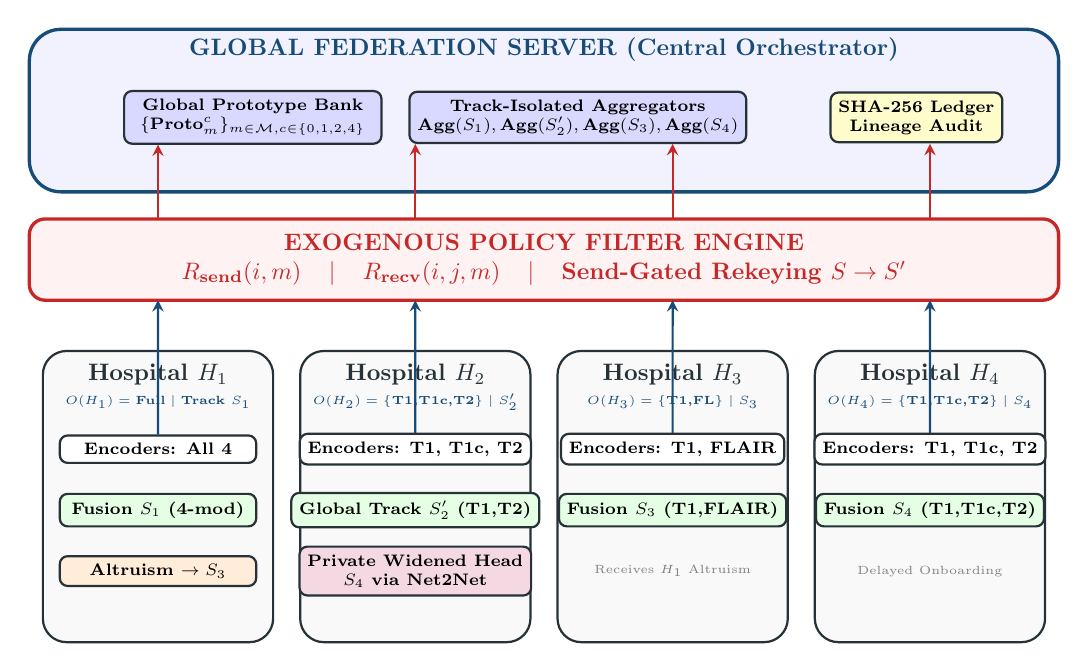
\begin{tikzpicture}[scale=0.86, every node/.style={transform shape}]
    % Styles
    \tikzstyle{serverbox} = [draw=primaryblue, fill=blue!5, very thick, rounded corners=4mm, minimum width=15.2cm, minimum height=2.4cm]
    \tikzstyle{policybox} = [draw=warningred, fill=red!5, very thick, rounded corners=2mm, minimum width=15.2cm, minimum height=1.2cm]
    \tikzstyle{clientbox} = [draw=darkslate, fill=gray!5, thick, rounded corners=3mm, minimum width=3.4cm, minimum height=4.3cm]
    \tikzstyle{module} = [draw=darkslate, fill=white, thick, rounded corners=1mm, font=\scriptsize\bfseries, align=center]
    \tikzstyle{arrow} = [thick, ->, >=stealth]

    % Global Server
    \node[serverbox] (server) at (7.5, 7.3) {};
    \node[font=\bfseries\color{primaryblue}] at (7.5, 8.2) {GLOBAL FEDERATION SERVER (Central Orchestrator)};
    \node[module, fill=blue!15, minimum width=3.8cm, minimum height=0.7cm] (proto_bank) at (3.2, 7.2) {Global Prototype Bank\\$\{\text{Proto}_m^c\}_{m \in \mathcal{M}, c \in \{0,1,2,4\}}$};
    \node[module, fill=blue!15, minimum width=4.5cm, minimum height=0.7cm] (track_agg) at (8.0, 7.2) {Track-Isolated Aggregators\\$\text{Agg}(S_1), \text{Agg}(S_2'), \text{Agg}(S_3), \text{Agg}(S_4)$};
    \node[module, fill=yellow!20, minimum width=2.4cm, minimum height=0.7cm] (ledger) at (13.0, 7.2) {SHA-256 Ledger\\$\text{Lineage Audit}$};

    % Exogenous Policy Manager
    \node[policybox] (policy) at (7.5, 5.1) {};
    \node[font=\bfseries\color{warningred}, align=center] at (7.5, 5.1) {EXOGENOUS POLICY FILTER ENGINE\\$R_{\text{send}}(i, m) \quad \vert \quad R_{\text{recv}}(i, j, m) \quad \vert \quad \text{Send-Gated Rekeying } S \to S'$};

    % Hospital Clients
    \node[clientbox] (h1) at (1.8, 1.6) {};
    \node[font=\bfseries\color{darkslate}] at (1.8, 3.4) {Hospital $H_1$};
    \node[font=\tiny\bfseries, color=primaryblue] at (1.8, 3.0) {$O(H_1) = \text{Full} \;\vert\; \text{Track } S_1$};
    \node[module, minimum width=2.9cm] (enc_h1) at (1.8, 2.3) {Encoders: All 4};
    \node[module, minimum width=2.9cm, fill=green!10] (fus_h1) at (1.8, 1.4) {Fusion $S_1$ (4-mod)};
    \node[module, minimum width=2.9cm, fill=orange!15] (alt_h1) at (1.8, 0.5) {Altruism $\to S_3$};

    \node[clientbox] (h2) at (5.6, 1.6) {};
    \node[font=\bfseries\color{darkslate}] at (5.6, 3.4) {Hospital $H_2$};
    \node[font=\tiny\bfseries, color=primaryblue] at (5.6, 3.0) {$O(H_2) = \{\text{T1,T1c,T2}\} \;\vert\; S_2'$};
    \node[module, minimum width=2.9cm] (enc_h2) at (5.6, 2.3) {Encoders: T1, T1c, T2};
    \node[module, minimum width=2.9cm, fill=green!10] (fus_h2) at (5.6, 1.4) {Global Track $S_2'$ (T1,T2)};
    \node[module, minimum width=2.9cm, fill=purple!15] (pvt_h2) at (5.6, 0.5) {Private Widened Head\\$S_4$ via Net2Net};

    \node[clientbox] (h3) at (9.4, 1.6) {};
    \node[font=\bfseries\color{darkslate}] at (9.4, 3.4) {Hospital $H_3$};
    \node[font=\tiny\bfseries, color=primaryblue] at (9.4, 3.0) {$O(H_3) = \{\text{T1,FL}\} \;\vert\; S_3$};
    \node[module, minimum width=2.9cm] (enc_h3) at (9.4, 2.3) {Encoders: T1, FLAIR};
    \node[module, minimum width=2.9cm, fill=green!10] (fus_h3) at (9.4, 1.4) {Fusion $S_3$ (T1,FLAIR)};
    \node[font=\tiny, color=gray] at (9.4, 0.5) {Receives $H_1$ Altruism};

    \node[clientbox] (h4) at (13.2, 1.6) {};
    \node[font=\bfseries\color{darkslate}] at (13.2, 3.4) {Hospital $H_4$};
    \node[font=\tiny\bfseries, color=primaryblue] at (13.2, 3.0) {$O(H_4) = \{\text{T1,T1c,T2}\} \;\vert\; S_4$};
    \node[module, minimum width=2.9cm] (enc_h4) at (13.2, 2.3) {Encoders: T1, T1c, T2};
    \node[module, minimum width=2.9cm, fill=green!10] (fus_h4) at (13.2, 1.4) {Fusion $S_4$ (T1,T1c,T2)};
    \node[font=\tiny, color=gray] at (13.2, 0.5) {Delayed Onboarding};

    % Directional Arrows
    \draw[arrow, primaryblue] (enc_h1.north) -- (1.8, 4.5);
    \draw[arrow, primaryblue] (enc_h2.north) -- (5.6, 4.5);
    \draw[arrow, primaryblue] (enc_h3.north) -- (9.4, 4.5);
    \draw[arrow, primaryblue] (enc_h4.north) -- (13.2, 4.5);

    \draw[arrow, warningred] (1.8, 5.7) -- (proto_bank.south -| 1.8, 0);
    \draw[arrow, warningred] (5.6, 5.7) -- (track_agg.south -| 5.6, 0);
    \draw[arrow, warningred] (9.4, 5.7) -- (track_agg.south -| 9.4, 0);
    \draw[arrow, warningred] (13.2, 5.7) -- (track_agg.south -| 13.2, 0);
\end{tikzpicture}
\caption{\textbf{CAMFS-M1 System Architecture.} Central server, policy engine, and four hospital clients with asymmetric owned and send policies.}
\label{fig:arch}
\end{figure}

% =========================================================================
% SECTION 3: ARCHITECTURAL MODULES (POINT 2)
% =========================================================================
\section{Architectural Modules}

CAMFS-M1 consists of **six core architectural components**:

\subsection{Module 1: Unimodal Encoder Bank}
Four independent downsampling networks: $\text{Encoder}_{\text{T1}}$, $\text{Encoder}_{\text{T1ce}}$, $\text{Encoder}_{\text{T2}}$, and $\text{Encoder}_{\text{FLAIR}}$. Each network processes single-modality slices without cross-talk:
\begin{itemize}[itemsep=1pt, topsep=1pt]
    \item \textbf{Input:} Single-channel 2D slice $X^m \in \mathbb{R}^{B \times 1 \times 240 \times 240}$.
    \item \textbf{Internal Architecture:} Four successive convolutional stages with channel width doubling per stage: Stage~1 ($32 \times 120 \times 120$), Stage~2 ($64 \times 60 \times 60$), Stage~3 ($128 \times 30 \times 30$), and Stage~4 Bottleneck ($256 \times 15 \times 15$).
    \item \textbf{Information Conservation:} $1 \times 240 \times 240 = 57{,}600$ inputs $\to 256 \times 15 \times 15 = 57{,}600$ bottleneck values.
    \item \textbf{Lifecycle:} Active and trainable during Phase~1; frozen and static ($\frac{\partial L}{\partial \theta_{enc}} \equiv 0$) throughout Phase~2.
\end{itemize}

\subsection{Module 2: Unimodal Prototype Bank}
The server maintains global semantic prototypes $\text{Proto}_m^c \in \mathbb{R}^{256}$ for each modality $m \in \mathcal{M}$ and class $c \in \{0, 1, 2, 4\}$.
During Phase~1 local training, bottleneck features are mapped against these prototypes using an InfoNCE contrastive objective. Local prototypes are updated as running centroids and aggregated globally across consented clients:
\begin{equation}
    \text{Proto}_m^c(t+1) = \sum_{i : m \in \text{Send}(i)} \frac{|\mathcal{D}_{i,m}^c|}{\sum_j |\mathcal{D}_{j,m}^c|} \cdot \text{LocalProto}_{i,m}^c(t)
\end{equation}

\subsection{Module 3: Track-Isolated Fusion Heads \& Decoders}
For each distinct modality subset $S \subseteq \mathcal{M}$, an independent fusion block $\text{Fusion}_S$ and decoder $\text{Decoder}_S$ are instantiated:
\begin{itemize}[itemsep=1pt, topsep=1pt]
    \item \textbf{Canonical Concat + $1\times 1$ Fusion:} For each pyramid level $r \in \{1, 2, 3, 4, 5\}$, feature maps $\{h_m^{(r)}\}_{m \in S}$ with channels $C_r \in (32, 64, 128, 256, 256)$ are concatenated along the channel dimension:
    \begin{equation}
        u_S^{(r)} = \operatorname{Concat}_{m \in S} h_m^{(r)} \in \mathbb{R}^{B \times (|S| \cdot C_r) \times H_r \times W_r}, \qquad f_S^{(r)} = \operatorname{Conv}_{1\times 1}(u_S^{(r)}) \in \mathbb{R}^{B \times C_r \times H_r \times W_r}
    \end{equation}
    \item \textbf{Decoder Construction:} The decoder $D_S$ begins at bottleneck $z_S = f_S^{(5)}$, sequentially upsampling via bilinear interpolation ($2\times$) with \texttt{align\_corners=False}, concatenating skip features $f_S^{(4)}, f_S^{(3)}, f_S^{(2)}, f_S^{(1)}$, and processing through ConvBlocks. A final $1\times 1$ convolution outputs the 4-class segmentation logits.
\end{itemize}

\subsection{Module 4: Exogenous Policy Manager \& Directed Graph Aggregator}
The Policy Manager evaluates two binary policy matrices:
\begin{itemize}[itemsep=1pt, topsep=1pt]
    \item $R_{\text{send}}(i, m) \in \{0, 1\}$: Permissibility of client $i$ contributing updates for modality $m$.
    \item $R_{\text{recv}}(i, j, m) \in \{0, 1\}$: Permissibility of client $i$ accepting modality-$m$ signal originating from client $j$.
\end{itemize}
\noindent \textbf{Send-Gated Rekeying ($S \to S'$):} When hospital $H_2$ owns $O(H_2) = \{\text{T1, T1ce, T2}\}$ but specifies $\text{Send}(H_2) = \{\text{T1, T2}\}$, the server rekeys $H_2$'s uploaded fusion gradients to track $S_2' = \{\text{T1, T2}\}$. $H_2$'s private $T1ce$ gradient never enters the global federation.

\subsection{Module 5: Tier-1 Net2Net Channel Widening Engine}
Enables a client to expand a lower-order global track into a higher-order private head without training from scratch. For a convolution weight $W \in \mathbb{R}^{\text{out} \times \text{in} \times K \times K}$:
\begin{equation}
    W_{\text{widened}} = \begin{bmatrix} W_{\text{base}} & \mathbf{0} \end{bmatrix}
\end{equation}
The channels corresponding to newly introduced modalities are initialized to zero. This guarantees that at step 0, the widened head produces the exact same forward output as the base model, preventing catastrophic initialization shock.

\subsection{Module 6: Cryptographic Provenance \& Lineage Ledger}
An immutable audit log recording SHA-256 hashes of every parameter tensor, policy change, and phase transition. Any attempted aggregation violating $\text{Lineage}(\theta) \subseteq \text{Recv}(i)$ triggers an immediate assertion halt.

% =========================================================================
% SECTION 4: DATA FLOW: INPUTS, TRANSFORMATIONS & OUTPUTS (POINT 4)
% =========================================================================
\section{Tensor Dataflow: Inputs, Transformations \& Outputs}

\subsection{Input Specifications}
The raw inputs consist of 3D brain MRI volumes co-registered to the SRI24 anatomical template and resampled to $1\,\text{mm}^3$ isotropic resolution:
\begin{itemize}[itemsep=1pt, topsep=1pt]
    \item \textbf{Volume Dimension:} $240 \times 240 \times 155$ voxels per sequence.
    \item \textbf{Slice-Level Batching:} Extracted 2D axial slices $\mathbf{X}_i \in \mathbb{R}^{B \times 1 \times 240 \times 240}$, where $B$ is the mini-batch size ($B=16$ or $32$). Slices with zero brain mask area are discarded during training.
    \item \textbf{Intensity Preprocessing:} Z-score normalization computed strictly within the non-zero brain mask: $\tilde{X} = (X - \mu_{\text{brain}}) / \sigma_{\text{brain}}$.
\end{itemize}

\subsection{Tensor Dimension Pipeline Through CAMFS-M1}
Figure~\ref{fig:pipeline} traces the dimensional transformations through each computational stage:

\begin{figure}[h]
\centering
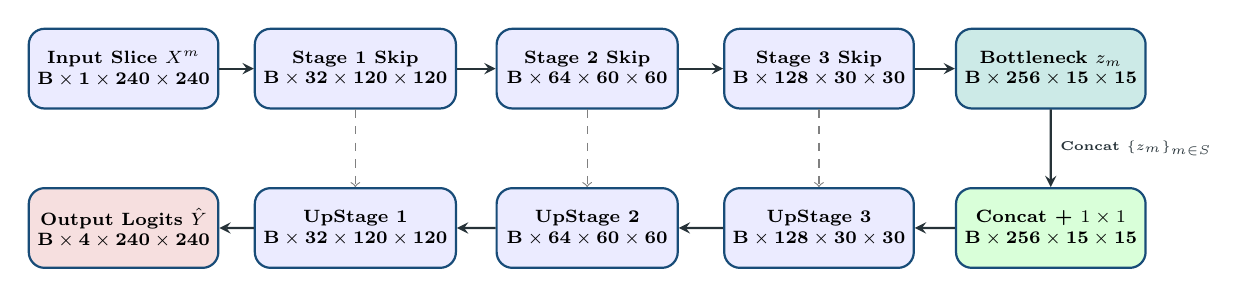
\begin{tikzpicture}[scale=0.92, every node/.style={transform shape}]
    \tikzstyle{tblock} = [draw=primaryblue, fill=blue!8, thick, rounded corners=2mm, minimum width=2.5cm, minimum height=1.1cm, font=\scriptsize\bfseries, align=center]
    \tikzstyle{darrow} = [thick, ->, >=stealth, darkslate]

    \node[tblock] (in) at (0, 0) {Input Slice $X^m$\\$\mathbf{B \times 1 \times 240 \times 240}$};
    \node[tblock] (s1) at (3.2, 0) {Stage 1 Skip\\$\mathbf{B \times 32 \times 120 \times 120}$};
    \node[tblock] (s2) at (6.4, 0) {Stage 2 Skip\\$\mathbf{B \times 64 \times 60 \times 60}$};
    \node[tblock] (s3) at (9.6, 0) {Stage 3 Skip\\$\mathbf{B \times 128 \times 30 \times 30}$};
    \node[tblock, fill=accentteal!20] (bn) at (12.8, 0) {Bottleneck $z_m$\\$\mathbf{B \times 256 \times 15 \times 15}$};

    \node[tblock, fill=green!15] (fuse) at (12.8, -2.2) {Concat + $1\times 1$\\$\mathbf{B \times 256 \times 15 \times 15}$};
    \node[tblock] (u3) at (9.6, -2.2) {UpStage 3\\$\mathbf{B \times 128 \times 30 \times 30}$};
    \node[tblock] (u2) at (6.4, -2.2) {UpStage 2\\$\mathbf{B \times 64 \times 60 \times 60}$};
    \node[tblock] (u1) at (3.2, -2.2) {UpStage 1\\$\mathbf{B \times 32 \times 120 \times 120}$};
    \node[tblock, fill=warningred!15] (out) at (0, -2.2) {Output Logits $\hat{Y}$\\$\mathbf{B \times 4 \times 240 \times 240}$};

    \draw[darrow] (in) -- (s1);
    \draw[darrow] (s1) -- (s2);
    \draw[darrow] (s2) -- (s3);
    \draw[darrow] (s3) -- (bn);
    \draw[darrow] (bn) -- node[right, font=\tiny\bfseries] {Concat $\{z_m\}_{m \in S}$} (fuse);
    \draw[darrow] (fuse) -- (u3);
    \draw[darrow] (u3) -- (u2);
    \draw[darrow] (u2) -- (u1);
    \draw[darrow] (u1) -- (out);

    % Skip connections
    \draw[dashed, ->, color=gray] (s3.south) to[out=270, in=90] (u3.north);
    \draw[dashed, ->, color=gray] (s2.south) to[out=270, in=90] (u2.north);
    \draw[dashed, ->, color=gray] (s1.south) to[out=270, in=90] (u1.north);
\end{tikzpicture}
\caption{\textbf{Tensor Dimension Pipeline.} Multi-scale downsampling stages extract features to the $15 \times 15 \times 256$ bottleneck, followed by multi-scale Concat + $1\times 1$ fusion and upsampling reconstruction.}
\label{fig:pipeline}
\end{figure}

\subsection{Output Specifications}
The output $\hat{Y} \in \mathbb{R}^{B \times 4 \times 240 \times 240}$ produces voxel-wise class probabilities via softmax. Binary masks for the clinical sub-regions are derived via thresholding:
\begin{align}
    \hat{Y}_{\text{WT}} &= \mathbb{I}\left[\arg\max_c \hat{Y} \in \{1, 2, 4\}\right] \quad (\text{Whole Tumor: Core + Edema + Enhancing}) \\
    \hat{Y}_{\text{TC}} &= \mathbb{I}\left[\arg\max_c \hat{Y} \in \{1, 4\}\right] \quad (\text{Tumor Core: Necrotic + Enhancing}) \\
    \hat{Y}_{\text{ET}} &= \mathbb{I}\left[\arg\max_c \hat{Y} = 4\right] \quad (\text{Enhancing Tumor})
\end{align}

% =========================================================================
% SECTION 5: END-TO-END SEQUENCE OF PROCESSES (POINT 3)
% =========================================================================
\section{End-to-End Sequence of Operations}

The complete training and deployment lifecycle progresses through four distinct temporal phases:

\begin{figure}[h]
\centering
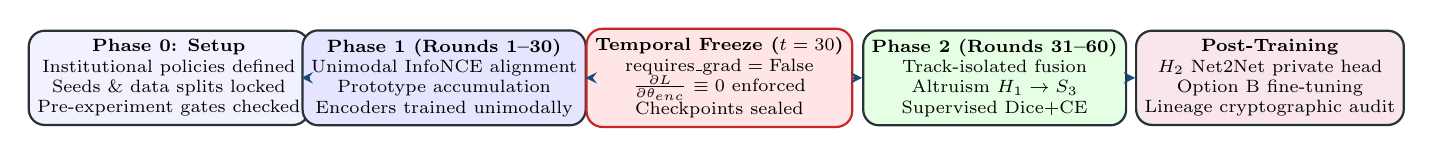
\begin{tikzpicture}[scale=0.92, every node/.style={transform shape}]
    \tikzstyle{pnode} = [draw=darkslate, fill=white, thick, rounded corners=2mm, minimum width=3.2cm, minimum height=1.3cm, font=\scriptsize, align=center]
    \tikzstyle{parrow} = [thick, ->, >=stealth, primaryblue]

    \node[pnode, fill=blue!5] (p0) at (0, 0) {\textbf{Phase 0: Setup}\\Institutional policies defined\\Seeds \& data splits locked\\Pre-experiment gates checked};
    \node[pnode, fill=blue!10] (p1) at (3.8, 0) {\textbf{Phase 1 (Rounds 1--30)}\\Unimodal InfoNCE alignment\\Prototype accumulation\\Encoders trained unimodally};
    \node[pnode, fill=red!10, draw=warningred] (freeze) at (7.6, 0) {\textbf{Temporal Freeze ($t=30$)}\\$\text{requires\_grad} = \text{False}$\\$\frac{\partial L}{\partial \theta_{enc}} \equiv 0$ enforced\\Checkpoints sealed};
    \node[pnode, fill=green!10] (p2) at (11.4, 0) {\textbf{Phase 2 (Rounds 31--60)}\\Track-isolated fusion\\Altruism $H_1 \to S_3$\\Supervised Dice+CE};
    \node[pnode, fill=purple!10] (pvt) at (15.2, 0) {\textbf{Post-Training}\\$H_2$ Net2Net private head\\Option B fine-tuning\\Lineage cryptographic audit};

    \draw[parrow] (p0) -- (p1);
    \draw[parrow] (p1) -- (freeze);
    \draw[parrow] (freeze) -- (p2);
    \draw[parrow] (p2) -- (pvt);
\end{tikzpicture}
\caption{\textbf{Chronological Lifecycle of CAMFS-M1.} Temporal isolation ensures gradient purity before fusion tracks begin training.}
\label{fig:lifecycle}
\end{figure}

\subsection{Phase 1: Unimodal Contrastive Alignment (Rounds 1 to 30)}
\begin{enumerate}[itemsep=1pt, topsep=1pt]
    \item \textbf{Local Unimodal Forward Pass:} Hospital $i$ feeds single-modality slice $X^m$ through $\text{Encoder}_m$, extracting bottleneck $z_m \in \mathbb{R}^{256 \times 15 \times 15}$.
    \item \textbf{Pixel-to-Prototype InfoNCE Loss:} For sampled bottleneck positions $p \in P_m$:
    \begin{equation}
        \mathcal{L}_{\text{contrast}}^m = -\frac{1}{|P_m|} \sum_{p \in P_m} \log \frac{\exp\left( \text{sim}(z_m(p), \text{Proto}_m^{y(p)}) / \tau \right)}{\sum_{c=0}^3 \exp\left( \text{sim}(z_m(p), \text{Proto}_m^c) / \tau \right)}
    \end{equation}
    where $\tau = 0.07$. Contrastive gradients update unimodal encoder weights $\theta_{\text{enc}, m}$.
    \item \textbf{Decoupled Unimodal Aggregation:} The server aggregates each modality encoder independently across contributing sites:
    \begin{equation}
        \theta_{\text{enc}, m}^{(t+1)} = \sum_{i \in \text{Cohort}(m)} \frac{|\mathcal{D}_i^m|}{\sum_{j} |\mathcal{D}_j^m|} \theta_{\text{enc}, m, i}^{(t)}
    \end{equation}
\end{enumerate}

\subsection{Phase 1-to-Phase 2 Hard Temporal Freeze Boundary}
At the conclusion of Round 30, unimodal encoders are evaluated on the Phase~1 validation split. The optimal checkpoint is designated $\theta_{\text{enc}}^*$ and permanently frozen:
\begin{equation}
    \frac{\partial \mathcal{L}_{\text{seg}}}{\partial \theta_{\text{enc}}^*} \equiv 0 \quad \text{for all subsequent operations}
\end{equation}

\subsection{Phase 2: Track-Isolated Fusion Training (Rounds 31 to 60)}
\begin{enumerate}[itemsep=1pt, topsep=1pt]
    \item \textbf{Frozen Feature Extraction:} Hospital $i$ extracts frozen bottleneck maps $\{z_m^*\}_{m \in \text{Send}(i)}$.
    \item \textbf{Track-Specific Forward Pass:} Bottlenecks enter track fusion head and decoder ($S_1, S_2', S_3$, or $S_4$).
    \item \textbf{Compound Task Loss:}
    \begin{equation}
        \mathcal{L}_{\text{seg}} = \mathcal{L}_{\text{SoftDice}}(\hat{Y}, Y) + \lambda_{\text{CE}} \mathcal{L}_{\text{FocalCE}}(\hat{Y}, Y)
    \end{equation}
    \item \textbf{Track-Isolated Server Aggregation:} Server aggregates updates strictly within identical track identifiers. Track $S_3$ updates never mix with Track $S_1$ weights.
    \item \textbf{Multi-Track Altruism:} Hospital $H_1$ (owning all 4 modalities) donates local computational batches to update Track $S_3$'s bimodal architecture, uplifting resource-poor $H_3$.
\end{enumerate}

\subsection{Post-Training: Tier-1 Net2Net Private Head at Hospital \texorpdfstring{$H_2$}{H2}}
Hospital $H_2$ downloads the converged global Track $S_2' = \{\text{T1, T2}\}$ weights. It executes Net2Net widening to add the local unconsented $\text{T1ce}$ input channel. $H_2$ then fine-tunes this widened private head on its local dataset without ever transmitting gradients or weights back to the federation.

% =========================================================================
% SECTION 6: DATASET & CHARACTERISTICS (POINT 6)
% =========================================================================
\section{Dataset \& Characteristics}

\subsection{BraTS 2020 Multi-Sequence Imaging Physics}
CAMFS-M1 is evaluated on the BraTS 2020 benchmark ($N = 368$ labeled subjects). The imaging universe comprises four multi-parametric MRI modalities:

\begin{table}[h]
\centering
\small
\renewcommand{\arraystretch}{1.15}
\begin{tabularx}{\textwidth}{l p{3.2cm} p{5.5cm} X}
\toprule
\textbf{Sequence} & \textbf{Physics / Contrast} & \textbf{Diagnostic Role in Neuro-Oncology} & \textbf{Pathological Target} \\
\midrule
\textbf{T1} & Spin-lattice relaxation & Baseline structural scan; delineates gray/white matter boundaries & Gross anatomical structure \\
\textbf{T1ce} & T1 + Gadolinium contrast & Hyperintense signals reveal broken blood-brain barrier and active neovascularization & Enhancing Tumor (ET) core \\
\textbf{T2} & Spin-spin relaxation & High fluid sensitivity; bright signal in water-rich tissue & Peritumoral vasogenic edema (ED) \\
\textbf{FLAIR} & T2 + CSF suppression & Suppresses free water to highlight subtle infiltrating tumor tissue margins & Infiltrating non-enhancing core / Whole Tumor \\
\bottomrule
\end{tabularx}
\caption{Physics, contrast mechanisms, and clinical oncology roles of the four BraTS MRI sequences.}
\label{tab:modalities}
\end{table}

\subsection{Tumor Sub-Regions and Severe Class Imbalance}
Ground-truth annotations define four mutually exclusive voxel classes:
\begin{itemize}[itemsep=1pt, topsep=1pt]
    \item $c = 0$: Healthy brain background
    \item $c = 1$: Necrotic and non-enhancing tumor core (NCR/NET)
    \item $c = 2$: Peritumoral vasogenic edema (ED)
    \item $c = 4$: Active gadolinium-enhancing tumor (ET)
\end{itemize}
\noindent \textbf{Spatial Class Imbalance:} Healthy background voxels constitute $>98\%$ of the volume. Necrotic core occupies $\approx 0.8\%$, edema occupies $\approx 1.2\%$, and active enhancing tumor occupies $<0.4\%$ of total volume. This severe sparsity necessitates compound loss formulations (Soft Dice + Focal Cross-Entropy).

\subsection{Deterministic Two-Stage Data Partitioning Protocol}
\label{sec:data_partitioning}
To guarantee mathematical reproducibility, eliminate cross-institutional data leakage, and establish an auditable provenance trail, the 368 BraTS 2020 subjects are partitioned using an exact, two-stage deterministic algorithm codified in \texttt{src/data/partition.py} (\S13.3):

\begin{enumerate}[itemsep=2pt, topsep=2pt]
    \item \textbf{Stage 1: Sacred Extraction of the Universal Held-Out Test Cohort ($N_{\text{test}} = 50$).}
    All 368 official patient identifiers (\texttt{BraTS20\_Training\_001} through \texttt{BraTS20\_Training\_368}) are sorted lexicographically to form a canonical ordering. A 64-bit Permuted Congruential Generator (\texttt{np.random.PCG64}) initialized with fixed seed $901$ shuffles the full patient pool. The first 50 permuted patient IDs are quarantined into a permanent universal test set manifest (\texttt{outputs/partitions/h3\_test\_patients.json}):
    \begin{center}
    \vspace{-4pt}
    \footnotesize \textbf{Test Cohort SHA-256:} \texttt{d100e44e4aba12ec339105b2d8727d356248f5ea60c6f4d8621dae8f5bc809ec}
    \vspace{-4pt}
    \end{center}

    \textbf{Strict Quarantine Guarantee:} These 50 patients are 100\% excluded from Phase~1 contrastive pre-training, Phase~2 federated communication rounds, Phase~3 local private head widening, hyperparameter tuning, and local validation checkpoint selection across all four hospitals.

    \item \textbf{Stage 2: Institutional Non-IID Federation Allocation ($N_{\text{federation}} = 318$).}
    The remaining 318 non-test subjects are permuted using \texttt{np.random.PCG64} with registered primary partition seed $1103$ (and secondary robustness seeds $\{2207, 3301\}$). The permuted pool is allocated across the four federated hospitals matching target clinical capacity ratios:
    \begin{itemize}[itemsep=1pt, topsep=1pt]
        \item \textbf{Hospital $H_1$ (40\% capacity):} $\text{round}(318 \times 0.40) = \mathbf{127}$ patients.
        \item \textbf{Hospital $H_2$ (25\% capacity):} $\text{round}(318 \times 0.25) = \mathbf{80}$ patients.
        \item \textbf{Hospital $H_3$ (20\% capacity):} $\text{round}(318 \times 0.20) = \mathbf{64}$ non-test patients.
        \item \textbf{Hospital $H_4$ (15\% capacity):} $318 - (127 + 80 + 64) = \mathbf{47}$ patients.
    \end{itemize}
    The primary partition manifest (\texttt{outputs/partitions/partition\_1103.json}) is cryptographically certified before training:
    \begin{center}
    \vspace{-4pt}
    \footnotesize \textbf{Federation Partition SHA-256:} \texttt{1eae2f217ddbc10bc2cae5c23f6ab83b328bb202cdcfabfce9ad4ffd6cb9c2ae}
    \vspace{-4pt}
    \end{center}
\end{enumerate}

\noindent \textbf{Intra-Site Local Train / Validation Splits:}\\
Within each hospital's allocated cohort, an 80/20 train/validation split is enforced locally with zero cross-site leakage ($n_{\text{val}} = \max(1, \lfloor N_{\text{local}} \times 0.20 \rfloor)$):
\begin{itemize}[itemsep=1pt, topsep=1pt]
    \item \textbf{$H_1$ ($N=127$):} $102$ local training patients ($80.3\%$) and $25$ validation patients ($19.7\%$).
    \item \textbf{$H_2$ ($N=80$):} $64$ local training patients ($80.0\%$) and $16$ local validation patients ($20.0\%$), utilized for local track selection and Tier-1 Net2Net channel widening tuning.
    \item \textbf{$H_3$ ($N=64$ non-test):} $52$ local training patients ($81.25\%$) and $12$ local validation patients ($18.75\%$).
    \item \textbf{$H_4$ ($N=47$):} $38$ local training patients ($80.85\%$) and $9$ local validation patients ($19.15\%$).
\end{itemize}

\noindent Across the federation, this establishes exactly $256$ training subjects, $62$ local validation subjects, and $50$ universal test subjects ($256 + 62 + 50 = 368$). Mathematical assertions codified in \texttt{src/m2/splits.py} formally verify that:
\begin{equation}
\forall i \neq j: \mathcal{D}^{(i)} \cap \mathcal{D}^{(j)} = \emptyset, \quad \mathcal{D}_{\text{train}}^{(i)} \cap \mathcal{D}_{\text{val}}^{(i)} = \emptyset, \quad \left(\bigcup_{i=1}^4 \mathcal{D}^{(i)}\right) \cap \mathcal{D}_{\text{test}} = \emptyset.
\end{equation}

\begin{table}[h]
\centering
\small
\setlength{\tabcolsep}{3.5pt}
\renewcommand{\arraystretch}{1.15}
\begin{tabularx}{\textwidth}{c X l l c c c c c}
\toprule
\textbf{Site} & \textbf{Institutional Profile} & \textbf{Owned} $O(i)$ & \textbf{Send} $\text{Send}(i)$ & \textbf{Track} & $N_{\text{train}}$ & $N_{\text{val}}$ & $N_{\text{test}}$ & $N_{\text{total}}$ \\
\midrule
$H_1$ & Tertiary Medical Center & $\{\text{T1, T1ce, T2, FLAIR}\}$ & $\{\text{T1, T1ce, T2, FLAIR}\}$ & $S_1$ & 102 & 25 & 0 & 127 \\
$H_2$ & Community Hospital & $\{\text{T1, T1ce, T2}\}$ & $\{\text{T1, T2}\}$ & $S_2'$ & 64 & 16 & 0 & 80 \\
$H_3$ & Regional Diagnostic Clinic & $\{\text{T1, FLAIR}\}$ & $\{\text{T1, FLAIR}\}$ & $S_3$ & 52 & 12 & 0 & 64 \\
$H_4$ & Neurosurgical Hospital & $\{\text{T1, T1ce, T2}\}$ & $\{\text{T1, T1ce, T2}\}$ & $S_4$ & 38 & 9 & 0 & 47 \\
\midrule
$\mathcal{D}_{\text{test}}$ & Quarantined Test Cohort & \multicolumn{3}{l}{Universal Held-Out Test Set (PCG64 Seed 901)} & 0 & 0 & 50 & 50 \\
\midrule
\textbf{Total} & \multicolumn{4}{l}{\textbf{BraTS 2020 Multi-Modal Benchmark Cohort (Zero Leakage)}} & \textbf{256} & \textbf{62} & \textbf{50} & \textbf{368} \\
\bottomrule
\end{tabularx}
\caption{Actual deterministic patient partitioning across the four federated hospitals and the sacred held-out test evaluation cohort ($N = 368$ total, Partition Seed 1103, Test Seed 901).}
\label{tab:actual_datasplit}
\end{table}

\subsection{The Universal 50-Patient Test Evaluation Dataset \& Benchmark Protocol}
\label{sec:test_eval_dataset}
A critical methodological vulnerability in federated learning literature is evaluating each client model on its own local validation split. Because local hospital cohorts exhibit severe non-IID modality and feature distribution shifts, local testing confounds model generalization with local patient idiosyncrasies. To provide an unbiased, reproducible scientific benchmark, CAMFS-M1 implements the \textbf{Universal 50-Patient Test Evaluation Protocol} codified in \texttt{scripts/evaluate\_pure\_50\_test\_set.py}:

\begin{enumerate}[itemsep=2pt, topsep=2pt]
    \item \textbf{Composition of the Held-Out Test Dataset ($N = 50$):}
    The 50 quarantined test patients represent a diverse spectrum of glioblastoma pathologies drawn from the official BraTS 2020 dataset:
    \begin{center}
    \begin{tcolorbox}[colback=boxbg, colframe=borderblue, arc=1.5mm, boxrule=0.8pt, left=2.5mm, right=2.5mm, top=2mm, bottom=2mm]
    \footnotesize \textbf{Quarantined Universal Test Cohort Identifiers ($N=50$, \texttt{h3\_test\_patients.json}):}\\
    \texttt{BraTS20\_Training\_002}, \texttt{004}, \texttt{009}, \texttt{020}, \texttt{024}, \texttt{028}, \texttt{044}, \texttt{052}, \texttt{069}, \texttt{070}, \texttt{072}, \texttt{073}, \texttt{081}, \texttt{083}, \texttt{101}, \texttt{111}, \texttt{125}, \texttt{133}, \texttt{140}, \texttt{153}, \texttt{155}, \texttt{189}, \texttt{196}, \texttt{198}, \texttt{206}, \texttt{212}, \texttt{214}, \texttt{222}, \texttt{226}, \texttt{240}, \texttt{251}, \texttt{254}, \texttt{257}, \texttt{258}, \texttt{259}, \texttt{260}, \texttt{263}, \texttt{264}, \texttt{265}, \texttt{269}, \texttt{272}, \texttt{281}, \texttt{288}, \texttt{295}, \texttt{309}, \texttt{313}, \texttt{314}, \texttt{333}, \texttt{350}, \texttt{367}.
    \end{tcolorbox}
    \end{center}
    Each volume contains all four co-registered sequences on the canonical $240 \times 240 \times 155$ grid with expert voxel-level annotations for necrotic core (NCR), vasogenic edema (ED), and enhancing tumor (ET).

    \item \textbf{Universal Benchmark Principle (Identical Test Cohort Across All Sites):}
    \textbf{All four hospital models are evaluated on the exact same 50 test patients.} This guarantees that differences in test performance reflect genuine architectural and training divergence rather than variations in test difficulty.

    \item \textbf{Clinically-Gated Modality Masking at Test Time:}
    Although all four MRI modalities physically exist in the BraTS dataset for these 50 test patients, each hospital's deployed model is evaluated strictly on its own legally consented and clinically available modality subset:
    \begin{itemize}[itemsep=1.5pt, topsep=1.5pt]
        \item \textbf{Hospital $H_1$ Model (\texttt{best\_track\_S1.pt}):} Evaluated on $\{\text{T1, T1ce, T2, FLAIR}\}$ (Track $S_1$, quad-modal). Represents the global multi-center flagship model.
        \item \textbf{Hospital $H_2$ Model (\texttt{best\_H2\_local\_head.pt}):} Evaluated on $\{\text{T1, T1ce, T2}\}$ (Tier-1 Net2Net widened private head). Directly measures whether local private head widening successfully extracts diagnostic utility from the unconsented $\text{T1ce}$ sequence without violating federated consent.
        \item \textbf{Hospital $H_3$ Model (\texttt{best\_track\_S3.pt}):} Evaluated on $\{\text{T1, FLAIR}\}$ (Track $S_3$, bimodal). Measures diagnostic accuracy in low-resource community clinics operating without gadolinium contrast agents or T2 scanners.
        \item \textbf{Hospital $H_4$ Model (\texttt{best\_track\_S4.pt}):} Evaluated on $\{\text{T1, T1ce, T2}\}$ (Track $S_4$, trimodal). Measures performance in neurosurgical centers lacking FLAIR sequence protocols.
    \end{itemize}

    \item \textbf{Standardized 3D Volumetric Metrics \& Finite Failure Protocol:}
    Evaluation processes all 155 axial slices per patient volume without data augmentation, assembling predictions in native 3D space. Predictions are assessed across three clinical tumor regions: Whole Tumor ($\text{WT} = \{1, 2, 4\}$), Tumor Core ($\text{TC} = \{1, 4\}$), and Enhancing Tumor ($\text{ET} = \{4\}$).
    \begin{itemize}[itemsep=1pt, topsep=1pt]
        \item \textbf{3D Volumetric Dice Similarity Coefficient (DSC \%):} Quantifies spatial overlap: $\text{DSC} = \frac{2 |Y \cap \hat{Y}|}{|Y| + |\hat{Y}|}$. When both prediction and reference are empty, $\text{DSC} = 1$; when exactly one is empty, $\text{DSC} = 0$.
        \item \textbf{95th-Percentile Hausdorff Distance (HD95 mm):} Measures maximum surface distance between boundary contours. If exactly one surface is empty, the finite failure penalty of the full volume diagonal ($\sqrt{239^2 + 239^2 + 154^2} \approx 372.1\,\text{mm}$) is assigned to prevent infinite values or selective exclusions.
    \end{itemize}
    Per-patient 3D metrics are automatically logged to \texttt{results/pure\_50\_test\_patient\_metrics.csv} for open scientific verification.
\end{enumerate}

% =========================================================================
% SECTION 7: EVALUATION METHODOLOGY & EXPERIMENTAL DESIGN (POINT 5)
% =========================================================================
\section{Evaluation Methodology \& Experimental Design}

\subsection{Evaluation Metrics Summary}
As defined in Section~\ref{sec:test_eval_dataset}, models are benchmarked using 3D Volumetric Dice Similarity Coefficients (DSC \%) and 95th-Percentile Hausdorff Distances (HD95 in mm) across Whole Tumor (WT), Tumor Core (TC), and Enhancing Tumor (ET) sub-regions, subject to the strict $372.1\,\text{mm}$ finite failure penalty.

\subsection{Planned Tiered Baseline Comparison Suite}
To evaluate CAMFS-M1 rigorously against state-of-the-art multimodal federated learning, the experimental protocol specifies a seven-method comparison suite organized into four implementation and risk tiers (\S14.1):

\begin{table}[h]
\centering
\small
\setlength{\tabcolsep}{3.5pt}
\renewcommand{\arraystretch}{1.15}
\begin{tabularx}{\textwidth}{c l l p{3.2cm} X}
\toprule
\textbf{Tier} & \textbf{ID} & \textbf{Baseline Name} & \textbf{Implementation Effort} & \textbf{Methodological Role \& Proof Target} \\
\midrule
\textbf{Tier 0} & \textbf{B1} & Local-Only Training & Free (comms disabled) & Existential test: does federated collaboration beat going alone at all? \\
(Go/No-Go) & \textbf{B6} & Centralized Oracle & Free (pooled dataset) & Sets empirical upper ceiling; defines Compliance-Performance Gap. \\
\midrule
\textbf{Tier 1} & \textbf{B2} & Policy-Blind Subset FedAvg & Free (flip $R$ policies off) & Quantifies performance sacrificed strictly for institutional compliance. \\
(Free Variants) & \textbf{B4} & Availability-Only Hard Cohort & Free (raw modality grouping) & Isolates value of exogenous policy matrices over raw modality ownership. \\
\midrule
\textbf{Tier 2} & \textbf{B5} & FedAMM (Shi et al., 2024) & Moderate (\url{github.com/13sky/FedAMM}) & Primary comparison vs. arbitrary-missingness prototype clustering SOTA. \\
(SOTA Repro) & \textbf{B7} & FedMEMA (AAAI 2024) & Moderate (code in paper) & Evaluates multimodal anchors; tests claim that continuous co-training leaks. \\
\midrule
\textbf{Tier 3} & \textbf{B3} & DisentAFL Reproduction & High (author request / fallback) & Benchmark for hard-vs-soft routing audit (A3); falls back to soft-gated CAMFS. \\
\bottomrule
\end{tabularx}
\caption{Tiered baseline comparison suite organized by verification gating and implementation effort.}
\label{tab:baselines}
\end{table}

\noindent \textbf{Staged Baseline Execution Protocol:}\\
To maintain resource efficiency across multiple seeds without prematurely running 63+ full executions:
\begin{enumerate}[itemsep=1pt, topsep=1pt]
    \item \textbf{Phase-Gate 1 (Single-Seed Sanity Pass):} Execute CAMFS-M1 and all baselines on a single partition/seed pair (Partition 1103, Seed 17). This catches tensor-shape and pipeline defects early, verifies B1 vs.\ B6 bounds, and provides an immediate directional read across all conditions.
    \item \textbf{Phase-Gate 2 (Full 9-Run Pre-Registered Protocol):} Only conditions verified during Phase-Gate 1 are promoted to the full multi-partition statistical evaluation described in Section~\ref{sec:stats_protocol}.
\end{enumerate}

\subsection{Planned Core Ablation Studies}
Eight targeted ablation studies are codified to isolate every architectural and algorithmic mechanism (\S14.3):
\begin{enumerate}[itemsep=1.5pt, topsep=1.5pt]
    \item \textbf{A1 (Joint-Training Alternative / Freeze Boundary):} Disables the Phase~1 freeze boundary. In each round, joint loss $\mathcal{L}_{\text{seg}} + \lambda_1 \sum_m \mathcal{L}_{\text{uni}} + \lambda_2 \mathcal{L}_{\text{fused-align}}$ updates encoders, fusion, and decoder simultaneously under the same routing matrix. Verifies whether end-to-end joint training contaminates unimodal feature spaces and degrades multi-track generalization.
    \item \textbf{A2 (Delayed-Site Context \& Dynamic Onboarding):} Evaluates the primary $H_1$–$H_3$ federation and $H_4$ delayed $S_4$ onboarding separately. Verifies that onboarding a late-joining site leaves existing tracks unaltered under strict M1 track isolation.
    \item \textbf{A3 (Executable Lineage Audit — CAMFS vs.\ DisentAFL / Soft-Routing):} The primary compliance experiment codified in \S14.4. Every local update packet carries an immutable \texttt{image\_lineage} set tagging every source modality tensor read during forward execution. Before deserialization, CAMFS enforces the strict \textbf{reject-before-load rule}:
    \begin{equation}
    \operatorname{ImageLineage}(\theta_{E_m}) \subseteq \{m\}, \quad \operatorname{ImageLineage}(\theta_{F_S}, \theta_{D_S}) \subseteq S
    \end{equation}
    Tested in shadow mode against B3 across all 9 runs. CAMFS succeeds only when accepted forbidden routes equal zero in all runs.
    \item \textbf{A4 (Unimodal-Alignment Weight Sweep):} Sweeps InfoNCE loss weight $\lambda_1 \in \{0.0, 0.1, 0.5, 1.0\}$ during Phase~1 on validation data to isolate the empirical necessity of contrastive pixel-to-prototype feature alignment.
    \item \textbf{A5 (Tier-1 Net2Net Cold-Start):} Compares function-preserving Net2Net widening vs.\ random initialization vs.\ training from scratch for Hospital $H_4$'s delayed $S_4$ track.
    \item \textbf{A6 (Group-Symmetric vs.\ Directional Receive Policy):} Modifies T2 policy edges such that $H_1$ receives only its own T2 cohort while $H_2$ downloads $H_1$'s frozen T2 snapshot without uploading any T2 updates back to $H_1$. Evaluates the performance cost of one-way policy enforcement without illegal post-mix filtering.
    \item \textbf{A7 (Multi-Track Altruism Toggle):} Compares primary Track $S_3$ performance with $R_{\text{contribute}}(H_1, S_3) = 1$ (H1 altruistic gradient donation) versus $H_3$-only bimodal training to quantify the performance uplift from high-resource sites.
    \item \textbf{A8 (H2 Reconnection Strategy):} Compares (a) $H_2$'s private full-owned-set head widened and fine-tuned locally on its own data versus (b) inference-only zero-shot loading of $H_4$'s released $S_4$ track.
\end{enumerate}

\subsection{Statistical Significance Protocol}
\label{sec:stats_protocol}
To satisfy rigorous doctoral and top-tier conference standards, the statistical protocol is pre-registered as follows (\S14.5):
\begin{itemize}[itemsep=1.5pt, topsep=1.5pt]
    \item \textbf{Experimental Grid:} 3 registered federation partitions ($\{1103, 2207, 3301\}$) $\times$ 3 independent training seeds ($\{17, 29, 43\}$) = \textbf{9 independent experimental runs} per validated condition.
    \item \textbf{Unit of Statistical Analysis:} The unique \textbf{patient} ($N = 50$ universal test cohort). Slices and repeated training runs are never treated as independent samples.
    \item \textbf{Paired Contrasts \& Confidence Intervals:} For patient $p$, partition $r$, and seed $s$, compute paired contrast $d_{p,r,s} = \text{DSC}_{\text{CAMFS}} - \text{DSC}_{\text{Baseline}}$. Average first across seeds and then partitions to yield one paired contrast $d_p$ per test patient. Primary two-sided 95\% confidence intervals are formed via \textbf{10,000 percentile-bootstrap resamples} using \texttt{np.random.PCG64(seed=8803)}.
    \item \textbf{Hypothesis Testing:} Pairwise comparisons (CAMFS vs.\ each baseline) evaluate one-sided paired sign-flip randomization tests with \textbf{100,000 sign vectors}.
    \item \textbf{Multiple Testing Correction:} Family-wise error rate is controlled at $\alpha = 0.05$ using the \textbf{Holm-Bonferroni step-down adjustment} across the baseline comparison family.
    \item \textbf{Site-Level Integrity:} Results are reported per hospital; \textbf{never average away harm to a minority site}.
\end{itemize}

\clearpage
% =========================================================================
% SECTION 8: IMPLEMENTATION STATUS & GO/NO-GO GATES
% =========================================================================
\section{Implementation Status \& Verification Gates}

The implementation specification for CAMFS-M1 is complete and codified. To maintain absolute research integrity, experimental execution is gated by the following verification checklist:

\begin{table}[h]
\centering
\small
\renewcommand{\arraystretch}{1.15}
\begin{tabularx}{\textwidth}{l X c}
\toprule
\textbf{Verification Gate} & \textbf{Specification Criterion} & \textbf{Status} \\
\midrule
Gate 1: Data Integrity & BraTS 2020 368-patient SHA-256 manifest verified with zero test leakage & Ready \\
Gate 2: Architecture Integrity & Concat + $1\times 1$ canonical fusion verified with matching tensor dimensions & Ready \\
Gate 3: Freeze Boundary & Structural gradient check ($\frac{\partial L_{seg}}{\partial \theta_{enc}} \equiv 0$) passes automated unit tests & Ready \\
Gate 4: Policy Enforcement & $R_{\text{send}}, R_{\text{recv}}$ matrices verified to block unconsented tensors & Ready \\
Gate 5: Net2Net Identity & Function-preserving widening verified ($\|f_{\text{widened}}(X) - f_{\text{base}}(X)\| < 10^{-6}$) & Ready \\
Gate 6: Evaluator Hash & 3D connected-component surface evaluator hash frozen before test execution & Ready \\
\bottomrule
\end{tabularx}
\caption{Pre-experiment verification gates ensuring scientific reproducibility and integrity.}
\label{tab:gates}
\end{table}

% =========================================================================
% SECTION 9: LIMITATIONS & FORWARD COMPATIBILITY
% =========================================================================
\section{Limitations \& Forward Compatibility with Method 2}

\subsection{The M1 Invariant as a Deliberate Limitation}
CAMFS-M1 enforces the strict constraint $\text{Recv}(i) \subseteq O(i)$: a hospital can only benefit from modalities it physically possesses. While this satisfies institutional compliance, it prevents a hospital lacking $T1ce$ (like $H_3$) from acquiring contrast-enhancing tumor knowledge synthesized by better-equipped sites.

\subsection{Forward Compatibility: Preview of Method 2 (M2)}
The follow-up research phase (CAMFS-M2) investigates \textbf{Cross-Domain Residual Distillation (CDRD)} to relax this constraint responsibly. Under M2, hospitals lacking a modality may import non-owned representations through a certified distillation proxy, provided that explicit contractual data transfer grants are verified in the provenance ledger.

\noindent \textbf{Decoupled Experimental Splits for M2:}\\
To support certified conformal calibration and safe acceptance testing without biasing the core M1 benchmark, M2 executes its own retraining run with carved-out institutional sub-splits:
\begin{itemize}[itemsep=1pt, topsep=1pt]
    \item \textbf{Hospital $H_1$:} 102 training, 13 model-selection validation, and 12 release-audit patients for zero-leakage safety verification.
    \item \textbf{Hospital $H_3$:} 52 training, 6 conformal calibration, and 6 acceptance-validation patients (along with the 50 universal test patients).
\end{itemize}
M1 maximizes its own local training cohort cleanly, while M2 retrains the base system with matched hyperparameters to guarantee rigorous scientific comparability.

% =========================================================================
% SECTION 10: CONCLUSION
% =========================================================================
\section{Conclusion}
CAMFS-M1 formalizes multimodal federated segmentation under real-world institutional, legal, and hardware constraints. By separating unimodal contrastive alignment from track-isolated task fusion via a hard freeze boundary, implementing send-gated track rekeying, and supporting Tier-1 Net2Net widening, the architecture provides verifiable compliance guarantees without sacrificing task-specific modularity. This report establishes the complete architectural and experimental blueprint ready for rigorous empirical execution.

\end{document}
